Las gráficas muestran un pulso triangular f y una sucesión periódica g de esos pulsos. Sean \(a,h>0\) y \(b>2a\); ambas funciones son cero para t<0. Los ejes y vértices fijan la altura h, la anchura 2a y el periodo b.
\begin{center}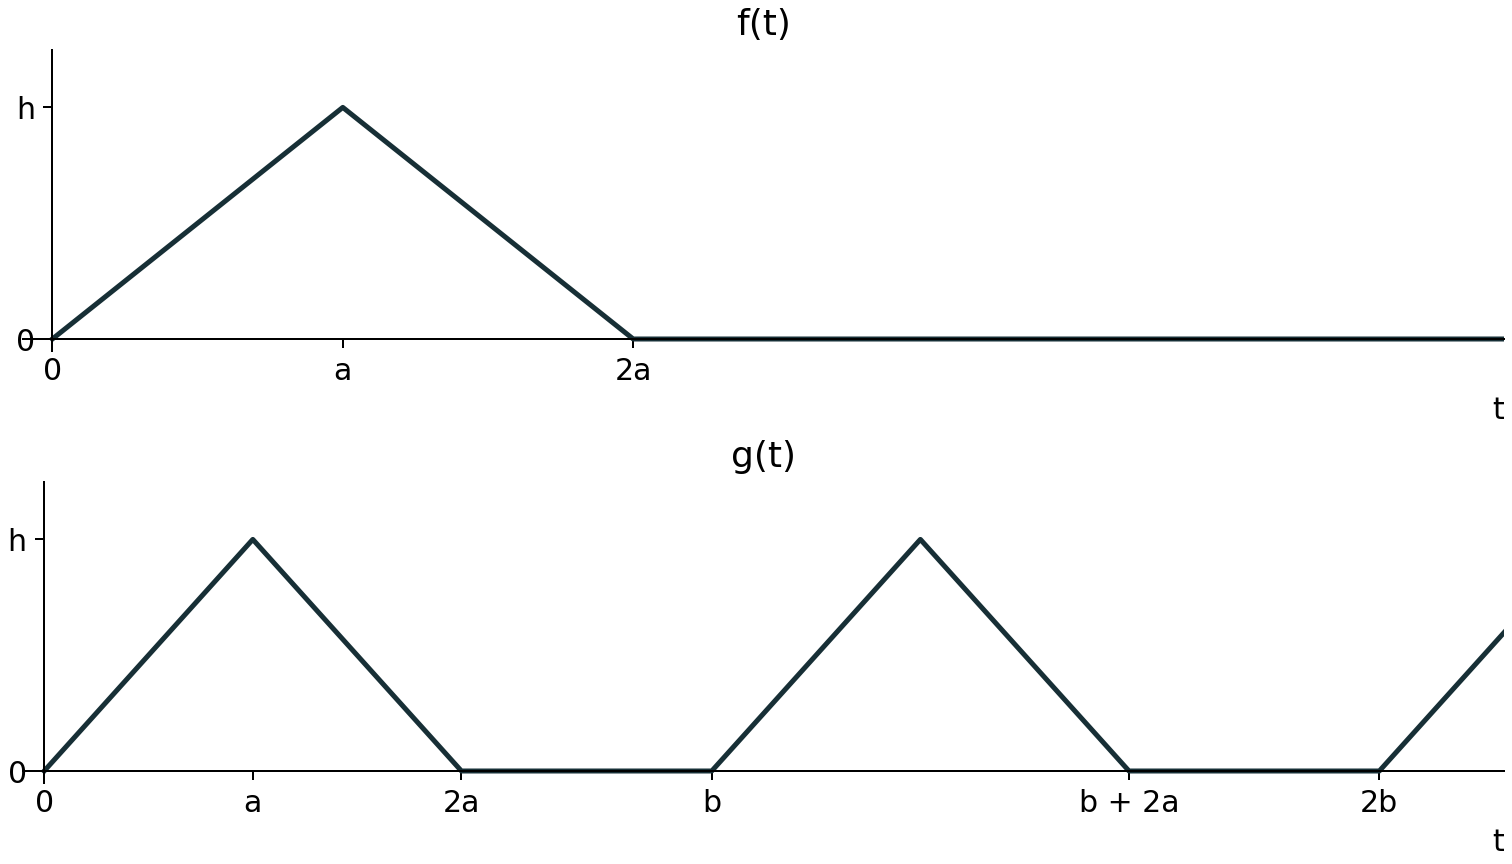
\includegraphics[width=.95\linewidth]{assets/M2-E0125-input.png}\end{center}

\begin{enumerate}[label=(\alph*),ref=\alph*,leftmargin=*]
\item Calcula la transformada de f.
\item Calcula la transformada de g.
\item Toma \(a=1\), \(h=4\) y resuelve \(y'+2y=f(t)\), \(y(0)\)=0.
\end{enumerate}
